

\section{Model Formulation \& overall approach}
\label{sec:approach}

\begin{figure}[t]
  \centering
  % Requires \usepackage{graphicx}
  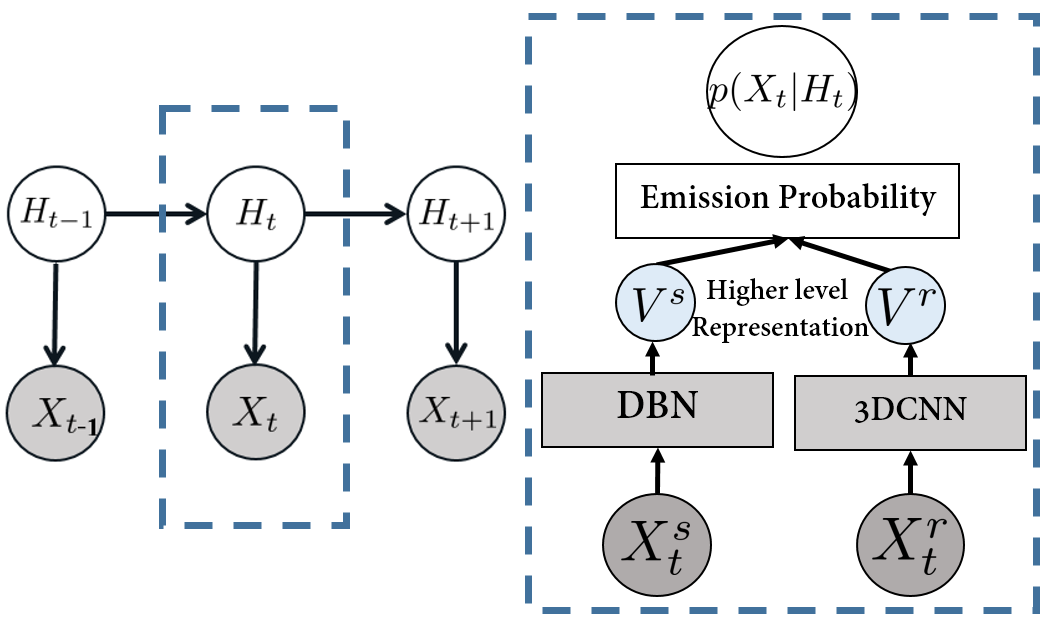
\includegraphics[width=0.45\textwidth]{images/GraphicalModel_new2}\\
  \caption{
 \small{ Gesture recognition model: the temporal model is a HMM (left), whose emission probability
\emissionprob{} (right) is modeled by forward-linked neural networks.
%%
More precisely, observations $\observation_t$ (skeletal features $\observationSK_t$, or RGB-D image features $\observationRGBD_t$)
are first passed through appropriate deep neural nets (a Deep Belief Network -\DBN- pretrained with Gaussian-Bernouilli Restricted Boltzmann Machines
for the skeleton modality, and
 a 3D convolutional neural network -\ThreeDCNN- for the \RGBD  modality) to implictly extract high-level features (\highSK and \highRGBD)
which are further fused to produce an estimate of $p(\observation_t|\hiddenstate_t)$.
}}
\label{fig:GM}
\end{figure}

Inspired by the framework successfully applied to speech recognition~\cite{mohamed2012acoustic}, the proposed model is a data driven learning system. This results in an integrated model, where the amount of prior knowledge and engineering is minimised. On top of that, this approach works without the need for additional complicated preprocessing and dimensionality reduction methods as it is naturally embedded in the framework.

The proposed approach relies on a Hidden Markov Model (HMM) for the temporal part,
and neural networks to model the emission probabilities.
 In the remainder of this section, we will first present our temporal model and then introduce its main component.
The details of the two distinct neural networks and fusion mechanisms along with post-processing will be provided
in Section~\ref{sec:ModelImplementation}.


\subsection{Deep Dynamic Neural Networks}
\label{sec:DDNN}

The proposed deep dynamic neural network \emph{(DDNN)} can be seen as an extension of~\cite{diwucvpr14}, where instead of only using the restricted Boltzmann machines to model human motion, various connectivity layers (fully connected layers, convolutional layers) are stacked together to learn higher level features justified by a variational bound~\cite{hinton2006fast} from different input modules.

A continuous-observation HMM  is adopted for modelling higher level temporal relationships.
At each time step $t$, we have one observed random variable $\observation_t$
composed of the skeleton input $\observationSK_t$ and RGB-D input images $\observationRGBD_t$
as shown in the graphical representation in Fig.~\ref{fig:GM}.
%
 The hidden state variable $\hiddenstate_t$ takes on values in a finite set  \finiteset composed of \numberhiddenstate states related to
the different gestures.
 The intuition motivating the HMM model is that a gesture is composed of a sequence of poses where the relative duration of each pose may vary.
This variance is captured by allowing flexible forward transitions within a Markov chain.
In practice,  $\hiddenstate_t$ can be interpreted as being in a particular phase  of a gesture \gesturea{}.

Classically under the HMM assumption, the joint probability of observations and states is given by:
\begin{equation}
p(H_{1:T},X_{1:T}) = p(H_1)p(X_1 | H_1) \prod^{T}_{t=2} p(X_t | H_t ) p(H_t | H_{t-1}),
\label{HMM_GM_1}
\end{equation}
where $p(\hiddenstate_1)$ is the prior on the first hidden state, $p(\hiddenstate_t|\hiddenstate_{t-1})$
is the transition dynamics modelling the allowed state transitions and their probabilities,
 and $p(\observation_t | \hiddenstate_t )$ is the emission probability of the observation,
modelled by  deep neural networks in our case. These elements are presented below.


%\subsection{Ergodic States Hidden Markov Model}

\begin{figure}[t]
  \centering
  % Requires \usepackage{graphicx}
  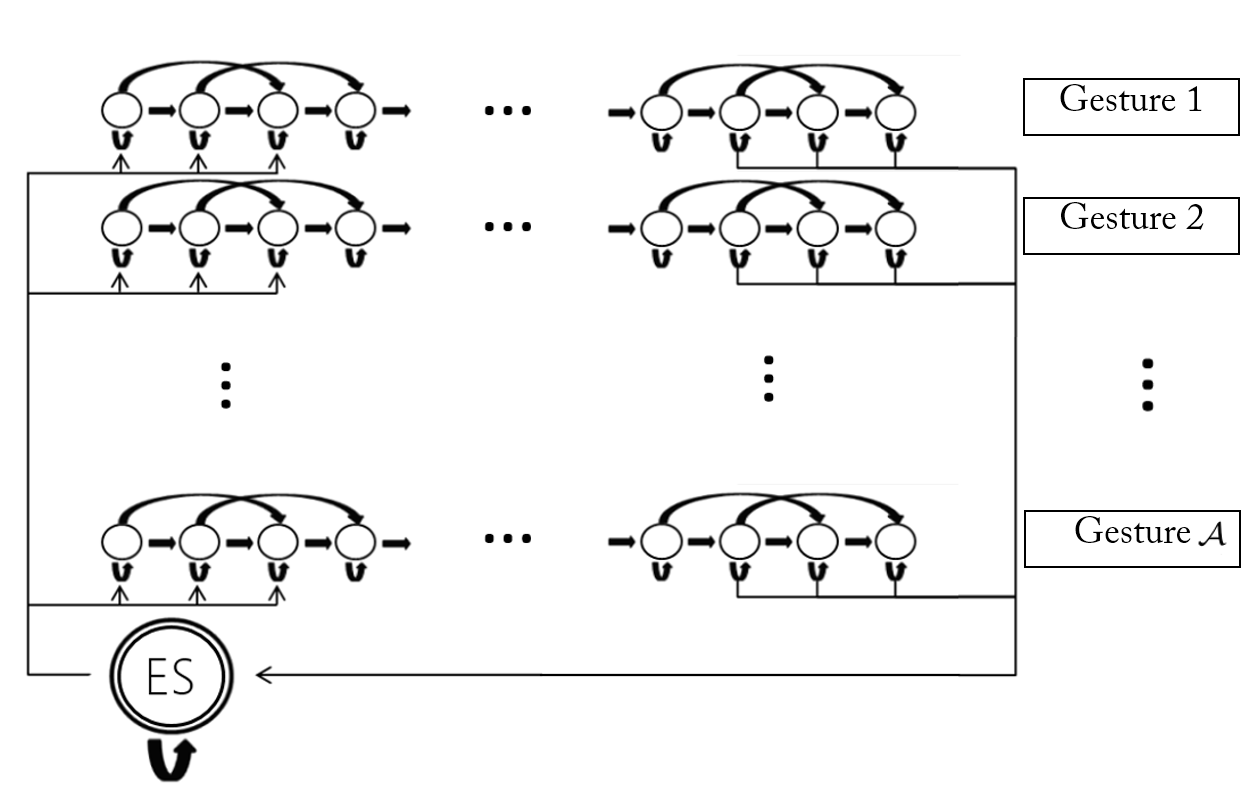
\includegraphics[width=0.45\textwidth]{images/HMM_2_new}\\
  \caption{
   \small{ State diagram of the \emph{ES-HMM} model for low-latency gesture segmentation and recognition. An ergodic state (\emph{$\mathcal{ES}$}) is used to model the resting position between gesture sequences. Each node represents a single state and each row represents a single gesture model. The arrows indicate possible transitions between states.}}
    \label{HMM_ES}
\end{figure}


\subsection{State-transition model and inference}
\label{sec:statemodel}


The HMM framework can be used for simultaneous gesture segmentation and recognition.
This is achieved by defining the state transition diagram as shown in Fig~\ref{HMM_ES}. For each given gesture $a \in \mathcal{A}$, a set of states $\mathcal{H}_a$ is introduced to defined a Markov model of that gesture. For example, for action sequence ``tennis serving", the action sequence can implictly be dissected into $\hiddenstatenode_{a_1}, \hiddenstatenode_{a_2}, \hiddenstatenode_{a_3}$ as: 1) raising one arm 2) raising the racket 3) hitting the ball.
More precisely, since our goal is to capture the variation in speed of the performed gestures, we set the transition matrix \transitionmatrix{}  in the following way: when being in a particular node $n$ at time $t$, moving to time $t + 1$, we can either stay in the same node (slower), move to node $n + 1$, or move to node $n+2$ (faster).
%
Furthermore, to allow the segmentation of gestures, we add an ergodic state
(\emph{$\mathcal{ES}$}) which resembles the silence state for speech recognition and which serve as a catch-all state.
From this state we can move to the first three nodes of any gesture class, and from the last three nodes of any gesture class we can move to $\mathcal{ES}$.
Hence, the hidden variable \hiddenvariable{} can take values within the finite set
 $\mathcal{H}=(\bigcup _{a \in \mathcal{A}} \mathcal{H}_a) \bigcup \{\mathcal{ES}\}$.

Overall, we refer to the model as the ergodic states hidden Markov model (\emph{ES-HMM}) for simultaneously gesture segmentation and recognition. It  differs from the firing hidden Markov model of~\cite{nowozin2012action} in that we strictly follow a left-right HMM structure without allowing backward transition, forbidding inter-states transverse, assuming that the considered gestures do not undergo cyclic repetitions as in walking for instance.


%The emission probability is represented as a matrix of size $N_{\mathcal{TC}} \times N_{\mathcal{F}}$ where $N_{\mathcal{F}}$ is the number of frames and output target class $N_{\mathcal{TC}}=N_{\mathcal{A}} \times N_{\mathcal{H}_a}+1$ where $N_{\mathcal{A}}$ is the number of gesture classes and $N_{\mathcal{H}_a}$ is the number of states associated to an individual gesture $a$ and one $\mathcal{ES}$ state (\emph{c.f.} Fig. \ref{Sample0700_comparison}: x-axis as $N_{\mathcal{F}}$ and y-axis as $N_{\mathcal{TC}} $ with $\mathcal{ES}$ as the bottom y-axis 101).


Once we have the trained model, we can use standard techniques to infer online the filtering
distribution $p(\hiddenstate_t | \observation_{1:t})$,  or offline (or with delay)
the smoothed distribution $p(H_t | X_{1:T})$ where $T$ denotes the end of the sequence.
Because the graph for the hidden Markov model is a directed tree, this problem can be solved exactly and efficiently using the max-sum algorithm also known as Viterbi algorithm. This algorithm searches the space of paths efficiently to find the most probable path with a computational cost that grows only linearly with the length of the chain~\cite{bishop2006pattern}.
%We can infer the gesture presence in a new sequence by Viterbi decoding.
% \begin{equation}
%    V_{t,\mathcal{H}}= \log P(X_t | H_t)+  \log(\max_{\mathcal{H} \in \mathcal{H}_a}( V_{t-1,\mathcal{H}}))
%    \label{viterbi_GDBN}
%\end{equation}
%whith the initial state $V_{1,\mathcal{H}}=P(X_1 |H_1)$.
%From the inference results, we define the probability of a gesture $a \in \mathcal{A}$ as $p(y_t=a|x_{1:t}) =V_{T,\mathcal{H}}$.
The result of the Viterbi algorithm is a path--sequence $\hat{\hiddenstatenode}_{t:T}$ of nodes going through the state diagram of
Fig.\ref{HMM_ES} and from which we can easily infer the class of the gesture as illustrated in Fig.~\ref{fig:Sample0700_comparison}.



\subsection{Learning the emission probability}
\label{sec:ProblemFormation}
\label{sec:emissionprob}

Traditionnally, emission probabilities for activity recognition have been trained with Gaussian Mixture Models (GMM), one per state.
%
Alternatively, in this work we propose to model this term in a discriminative fashion.
More precisely, since the input features have a high dimensionality,
we propose to learn them using two distinctive types of neural networks suited to the input modality,
as summarized in the right of Fig.~\ref{fig:GM}.
%
Unfortunately, estimating a probability density such as an emission probability remains quite a difficult problem, especially in high dimensions. However, inference in the HMM only depends only on the ratio between emission probabilities for the different states. Since training a model to predict a density ratio is often significantly easier, we will directly predict the ratio between emission probabilities. This is similar to the approach used by Kindermans et al. to integrate transfer learning and an HMM based language model into a single probabilistic model \cite{Kindermans2012a}.
One should think of the predicted emission probability ratio as an unnormalized version of the true emission probability. Nevertheless, to simplify the discussion of our models for readers with a basic understanding of HMMs, we will refer to the predicted emission probability ratio simply as emission probabilities since the underlying model remains unchanged.

For  the skeletal features, we rely on a Deep-Belief Network (DBN) trained in two steps \cite{salakhutdinov2009learning}:
in the first step,  stacked Restricted Boltzmann Machines (RBM) is trained in an unsupervised fashion using only observation data
to learn  high-level feature representations;
in the second step, the model is used as a Deep-Belief Network whose weights are further fine-tuned
for learning the emission probability.
%
For the RGB and depth (RGB-D) video data, we rely on a 3D (2D for space and 1D for time)
convolutional neural networks (3DCNN) to model the emission probabilities.
%
Finally, a fusion method combines in an intermediate or in a late stage the contributions of both modalities.
%
In all cases (including the fusion), the supervised training is conducted by learning to
predict the state label (an element of \finiteset) associated to each training or testing frame.


Such an approach present several advantages over the traditional GMM paradigm.
%
%Traditionally, GMMs and HMMs co-evolved as a way of doing speech recognition when computers were too slow to explore more computationally intensive approaches.
First, while  GMMs are easy to fit when they have diagonal covariance matrices and, with enough components,
can model any distribution, they have been shown to statistically inefficient at modeling high-dimensional features
with many componential structure as explained in~\cite{mohamed2012acoustic}.
%
For instance, assume that the components of the input feature space can be separated into two subspaces
characterized by  $N$  and $M$ significantly different  patterns in the training data, respectively, and that the occurences
of these patterns are relatively independent\footnote{In our case, intuitively these spaces could be the  features from different body parts,
like left/right arm or torso features.}.
%
A GMM will requires $N*M$ components to model this structure because each component must generate all the input features.
%
On the other hand, a stacked RBMs model that can explains the data using multiple causes only requires $N+M$ components
(in the ideal fully independent case), each of which is specific to a particular subspace.
%
This exponential inefficiency of GMMs at modeling factorial structures leads to GMM+HMM systems having
a very large number of Gaussians, most of which must be estimated from a very small fraction of the data.


Secondly, the approach for training the skeleton DBN model, first using variational learning to train stacked RBMs with unlabeled data, then in a discriminative fashion
\cite{salakhutdinov2009learning} has been shown to have several advantages.
%
It has been observed that  variational learning~\cite{hinton2006fast},
which tries to optimize the data-likelihood while minizing the Kullback-Leibler divergence between
the true posterior distribution of the hidden state (i.e. hidden layer variables of the RBMs  in our case)
and an approximation of this distribution, tends to produce unimodal distributions.
%
This is beneficial, as this means that similar sensory inputs will be mapped to  similar hidden variables.
%
Thus, the intuition for using DBN  for modeling the emission probability $p(\observation_t|\hiddenstate_t)$
from skeleton joints  is that by learning the multi-layer network layer by layer,
semantically meaningful high level features for skeleton configuration will be extracted while at the same
time a  parametric prior of human pose is learned.
%
%In the recent work of~\cite{6751269} a non-parametric bayesian network is adopted for human pose prior estimation, whereas in our framework, the parametric networks are incorporated.
%
In our case, using the pair wise joints features as raw input, the data-driven approach network will be able to extract relational
multi-joints features which are relevant to the target classes.
For instance, from  the ``toss" action data, a wrist joints rotating around shoulder joints feature is expected to
be extracted from the backpropagation  learning, and be the equivalent of those task specific \emph{ad hoc} hard wired sets
of joints configurations defined in~\cite{chaudhry2013bio}~\cite{muller2006motion}\cite{nowozin2012action}~\cite{ofli2013sequence}.

The benefit of such a learning approach is even more important when large amount of unlabelled data (e.g. skeleton data
 inferred from depth images of people performing unknown gestures) is available in addition to the labeled ones
(this was not the case in this paper).
%
%% The benefit of learning a generative model is greatly magnified when there is a large supply of unlabeled skeletal, RGB and depth data either acquired by motion capture systems or inferred from depth images in addition to the training data that has been labeled by a forced HMM alignment. We do not make use of unlabeled data in this paper, but it could only improve our results relative to purely discriminatively approaches.
%
Naturally, many of the  features learned in this unsupervised way might  be irrelevant for making the required discriminations,
even though they are important for explaining the input data.
However, this is a price worth paying if data availability and computation are cheap and
lead to  a stable mapping of the high-dimensional input  into high-level features
that are very good for discriminating between classes of interest.
%
In this view, it is important to notice that each weight in a neural network is usually constrained by a larger fraction of
the training samples than each parameter in a GMM, a point that has been masked by other differences in training.
In particular,  neural networks have traditionally been training discriminatively, whereas GMMs are typically trained as generative models,
%(even if discriminative training is performed later in the training procedure).
which given their parametric  nature  partially compensate the fact that each mixture
of a large GMM is usually trained on a very small fraction of the data.

In summary, the feed forward neural networks offer several potential advantages over GMMs:
\begin{itemize}
\item their estimation of emission  probabilities does not require detailed assumptions about the data distribution;
\item they allow an easy combination of diverse features, including both discrete and continuous features;
\item they use far more of the data to constrain each parameter because the output on each training case
is sensitive to a large fraction of the weights.
\end{itemize}



%% \textbf{Learning the higher level representation for skeleton joints features}: \label{skeleon_high_level}

%Neal and Hinton~\cite{neal1998view} demonstrated that the negative log probability of a single data vector, $\textbf{v}^0$, under the multi-layer generative model is bounded by a variational free energy, which is the expected energy under the approximating distribution, $Q(\textbf{h}^0 |\textbf{v}^0 )$, minus the entropy of that distribution. For a directed model, the ``energy" of the configuration $\textbf{v}^0 $,$\textbf{h}^0$ is given by $  E(\textbf{v}^0, \textbf{h}^0) = - [ \log p(\textbf{h}^0)+ \log p(\textbf{v}^0 | \textbf{h}^0)]$.
%% So the bound is
%% \begin{align*}
%%     \log p(\textbf{v}^0) &\geqslant \sum_{\textbf{h}^0} Q(\textbf{h}^0 | \textbf{v}^0) [ \log p (\textbf{h}^0) + \log p (\textbf{v}^0 | \textbf{h}^0)] \\
%%      &- \sum_{\textbf{h}^0} Q(\textbf{h}^0 | \textbf{v}^0) \log Q(\textbf{h}^0 |\textbf{v}^0)
%% \end{align*}

%% The intuition using deep belief networks for modeling marginal distribution \emissionprob{} in skeleton joints action recognition is that by constructing multi-layer networks, semantically meaningful high level features for skeleton configuration will be extracted whilst learning the parametric prior of human pose from mass pool of skeleton joints data. In the recent work of~\cite{6751269} a non-parametric bayesian network is adopted for human pose prior estimation, whereas in our framework, the parametric networks are incorporated.

%% Using the pair wise joints features as raw input, the data-driven approach network will be able to extract relational multi-joints features which are relevant to target frame class. E.g., for ``toss" action, wrist joints is rotating around shoulder joints would be extracted from the backpropagation via target frame as those task specific, \emph{ad hoc} hard wired sets of joints configurations as in~\cite{chaudhry2013bio}~\cite{muller2006motion}\cite{nowozin2012action}~\cite{ofli2013sequence}.

%% The outputs of the neural net are the hidden states learned by force alignment during the supervised training process.
%% Once we have model, we can use the normal online or offline smoothing, inferring the hidden marginal distributions of every node (frame) of the test video.

%The overall algorithm for training and testing are presented in Algorithm \ref{MMDDN_train} and \ref{MMDDN_test}.

%\begin{algorithm}
%\caption{Multimodal deep dynamic networks -- training}\label{MMDDN_train}
%\LinesNumbered
%\SetAlgoLined
%\SetAlgoNoEnd
%\DontPrintSemicolon
%\SetKwFunction{zeroes}{zeroes}
%\KwData{\;
%          \inputsequence=$[\framefeature_{i,1}, \ldots,\framefeature_{i,t},\ldots, \framefeature_{i,T}]$ \;
%          $ \mathbf{X^1=\{ x^1_i\}_{i \in [1 \ldots t]}}$ - raw input (skeletal) feature \; \hspace{1cm} sequence.\;
%          $ \mathbf{X^2=\{ x^2_i\}_{i \in [1 \ldots t]}}$ - raw input (depth) feature \; \hspace{1cm} sequence in the form of     $M_1 \times M_2 \times T$, where \; \hspace{1cm} $M_1, M_2$ are the height and width of the input \; \hspace{1cm} image and $T$  is the number of contiguous \; \hspace{1cm} frames of the spatio-temporal cuboid. \;
%          $ \mathbf{Y=\{ y_i\}_{i \in [1 \ldots t]}}$  - frame based local label (achieved by\; \hspace{1cm} semi-supervised forced-aligment), where \;
%          \hspace{1cm} $ \mathbf{y_i} \in \{ N_{\mathcal{A}} * N_{\mathcal{H}_a} + \textbf{\emph{1}} \} $ with $N_{\mathcal{A}}$ the number of \;
%          %\hspace{1cm} classes, $N_{\mathcal{H}_a$ is the number of hidden states for \; \hspace{1cm} each class,
%          \hspace{1cm} gesture classes and $N_{\mathcal{H}_a}$ is the number of \;
%          \hspace{1cm} states associated to an individual gesture $a$ \;
%          \hspace{1cm} and $\textbf{\emph{1}}$ as ergodic state.
%            }
%%\For{$m \leftarrow 1$ to $2$}{
%    \SetAlgoVlined
%    %\eIf{$m$ is $1$}{
%
%
%        Preprocess skeletal data $ \mathbf{X^1}$ as in Eq.\ref{sk_features_1}, \ref{sk_features_2}, \ref{sk_features_3}.\;
%        Normalise (zero mean, unit variance per dimension) the above features and feed it to Eq.\ref{GRBMenergy}. \;
%        Pre-train the networks using \emph{Contrastive Divergence}. \;
%        Supervised fine-tuning of the deep belief networks using $ \mathbf{Y}$ by standard mini-batch \emph{SGD} backpropagation.\;
%    %}{
%        Preprocess the depth and RGB data $ \mathbf{X^2}$ as in \ref{3d_preproc}.\;
%        Feed the above features to Eq.\ref{ReLU}. \;
%        Train the 3D convolutional neural networks using $ \mathbf{Y}$.\;
%    %}
%%}
%\KwResult{\;
%        $\mathbf{GDBN}$ - a Gaussian-Bernoulli visible layer deep \;
%                \hspace{1cm} belief network to generate the emission \;
%                \hspace{1cm} probabilities for the hidden Markov model.\;
%        $\mathbf{3DCNN}$ - a 3D deep convolutional neural \;
%                    \hspace{1cm} network to generate the emission probabilities\;
%                    \hspace{1cm} for the hidden Markov model.\;
%        $\mathbf{p(X_t | H_t )}$ emission probability. \;
%        $\mathbf{p(H_1)}$ - prior probability for $ \mathbf{Y}$ by accumulating and \;
%                \hspace{1cm} normalising labels.\;
%        $ \mathbf{p(H_t | H_{t-1})}$ - transition probability for $ \mathbf{Y}$,  enforcing\;
%                \hspace{1cm} the beginning and ending of a sequence can \;
%                \hspace{1cm} only start from the first or the last state.
%}
%\end{algorithm}
%%%%%%%%%%%%%%%%%%%%%%%%%%%%%%%%%%%%%%%%%%%%%%%%%%%%%%%%%%%%%%%%%%%%%%%%%%%%%%%%%%%%%%%%%%%%%%%%%%%%%%%%%%%%%%%%%
%\begin{algorithm}[t]
%\caption{Multimodal deep dynamic networks -- testing}\label{MMDDN_test}
%\LinesNumbered
%\SetAlgoLined
%\SetAlgoNoEnd
%\DontPrintSemicolon
%\SetKwFunction{zeroes}{zeroes}
%\KwData{\;
%         $\mathbf{X^1=\{x^1_i\}_{i \in [1 \ldots t]}}$ - raw input (skeletal) feature \; \hspace{1cm} sequence.\;
%         $\mathbf{X^2=\{x^2_i\}_{i \in [1 \ldots t]}}$ - raw input (depth) feature \; \hspace{1cm} sequencein the form of $M_1 \times M_2 \times T$. \;
%         $\mathbf{GDBN}$ - trained Gaussian-Bernoulli visible layer  \;
%                \hspace{1cm} deep belief network to  generate the emission\;
%                 \hspace{1cm} probabilities for the hidden Markov model.\;
%         $\mathbf{3DCNN}$ - trained  3D deep convolutional neural\;
%                    \hspace{1cm} network to generate the emission\;
%                    \hspace{1cm} probabilities for the hidden Markov model.\;
%        $\mathbf{p(H_1)}$ - prior probability for $ \mathbf{Y}$.\;
%        $ \mathbf{p(H_t | H_{t-1})}$ - transition probability for $ \mathbf{Y}.$
%            }
%
%%\For{$m \leftarrow 1$ to $2$}{
%    \SetAlgoVlined
%    %\eIf{$m$ is $1$}{
%        Preprocessing and normalising the skeletal data $ \mathbf{X^1}$  as in Eq. \ref{sk_features_1}, \ref{sk_features_2}, \ref{sk_features_3}.\;
%        Feedforwarding network $\mathbf{GDBN}$ to generate the emission probability $\mathbf{p(X_t | H_t )}$ in Eq.\ref{HMM_GM_1}. \;
%        Generating the score probability matrix $\mathbf{S^1 = p(H_{1:T},X_{1:T}).}$ \;
%    %}{
%        Preprocessing(median filtering the depth data) and normalising data RGB-D data $ \mathbf{X^2}$ .\;
%        Feedforwarding $\mathbf{3DCNN}$ to generate the emission probability $\mathbf{S^2 = p(X_t | H_t )}$ in Eq.\ref{HMM_GM_1}. \;
%        Generating the score probability matrix $\mathbf{S^2 =p(H_{1:T},X_{1:T}).}$ \;
%    %}
%%}
%        Fuse the score matrix $\mathbf{S = \alpha * S^1 + (1-\alpha)* S^2}$ OR the learnt joint representation.\;
%        Finding the best path $\mathbf{V_{t,\mathcal{H}}}$ using $\mathbf{S}$ by Viterbi decoding. \;
%\KwResult{\;
%        $ \mathbf{Y=\{ y_i\}_{i \in [1 \ldots t]}}$  - frame based local label  \;
%        $ \mathbf{C}$ - global label, the anchor point is chosen as the\;
%                        \hspace{1cm} middle state frame.\;
%}
%\end{algorithm}



\endinput
